\documentclass[11pt,a4paper]{article}
\usepackage[utf8]{inputenc}
\usepackage[T1]{fontenc}
\usepackage{amsmath,amssymb}
\usepackage{booktabs}
\usepackage{longtable}
\usepackage{graphicx}
\usepackage{float}
\usepackage[round,authoryear]{natbib}
\usepackage{hyperref}
\usepackage[margin=25mm]{geometry}
\usepackage{array}
\usepackage{xcolor}

\hypersetup{colorlinks=true,linkcolor=blue!60!black,citecolor=green!50!black,urlcolor=blue!70!black}
\setlength{\parskip}{0.45em}
\setlength{\parindent}{0pt}
\sloppy

\title{Novelty Assessment:\\
       Delay--Layout Coupling in UWB Self-Calibration\\[5pt]
       \large Prior-Art and Identifiability Analysis (Paper~B: Mechanism)}
\author{Zekai Xiao}
\date{June 2026}

\begin{document}
\maketitle

\section{One-Sentence Thesis}

UWB anchor self-calibration couples antenna-delay/range-bias parameters with layout scale, which makes same-environment tag accuracy unreliable as a calibration-quality metric. In the Erlangen campaign the \texttt{v4-io} layout is scale-biased (metric-incorrect): an under-absorbed common-mode range bias expands it to an AutoPos-to-Vicon Sim(3) scale of 0.958---this is a range-bias signature, not a true geometric distortion. This scale-biased layout gives a better static median (72.7~mm) than the metric-correct common-mode layout (109.5~mm) \emph{only when the tag delay is uncorrected}, because the layout's scale bias compensates an uncorrected positive tag-device delay. The effect is conditional: once the tag delay is corrected with a single global constant the metric-correct layout becomes the better positioner (68.5~mm held-out median, P95 156~mm, versus the scale-biased layout's 72.7~mm; better at 17 of 24 positions, paired $p\approx0.02$, though the marginal-median gap alone is within noise), so the claim is not that a metric-incorrect layout is inherently a better positioner, but that same-environment accuracy can rank a scale-biased layout above an independently validated metric-correct one when a correctable tag/range bias is left uncorrected.

\section{What the Full Text Confirms}

\subsection{UWB Self-Calibration}

The UWB self-calibration literature already treats anchor deployment as a major cost and addresses automatic anchor localization from radio measurements, robot trajectories, multihop constraints, or auxiliary sensing. Hamer and D'Andrea derive a self-calibrating UWB network for multi-robot localization, including clock synchronization and anchor position computation \citep{hamer_2018_self_calibrating_ultra_wideband_network}. Ledergerber, Hamer, and D'Andrea show a one-way UWB robot self-localization system \citep{ledergerber_2015_robot_self_localization_one_way_uwb}. Almansa et al. study mobile UWB autocalibration for ad-hoc robot deployments, while Corbalan et al. evaluate large-scale UWB anchor self-localization in practical multihop testbeds \citep{almansa_2020_autocalibration_mobile_uwb_localization,corbalan_2023_self_localization_uwb_anchors}. Van Herbruggen et al. and related self-calibration work address multihop or collaborative anchor positioning \citep{herbruggen_2023_multihop_self_calibration_algori,ridolfi_2021_self_calibration_and_collaborati,shi_2019_anchor_self_localization_algorit}. These papers are close in deployment motivation, but their success metric is usually localization or anchor reconstruction after calibration. They do not report the paradox that a scale-biased layout can outperform a metric-correct one because of tag-side NLOS cancellation.

Lutz et al. are the closest methodological prior art because their full text explicitly calibrates both UWB anchor poses and a UWB sensor error model using visual-inertial SLAM and fiducial markers \citep{lutz_2019_visual_inertial_slam_uwb_error_model}. Their problem formulation acknowledges that radio propagation makes a consistent sensor error model difficult across anchor setups. That is close to our concern, but the estimator is aided by VINS/AprilTags and does not expose the scale--delay coupling of range-only anchor self-calibration or the in-environment cancellation that lets the scale-biased layout outperform the metric-correct one.

\subsection{Antenna Delay, Range Bias, and Error Models}

The antenna-delay and range-bias literature is extensive and directly relevant. Shalaby et al. propose a robust antenna-delay calibration procedure and model bias/uncertainty as a function of received-signal power \citep{shalaby_2023_calibration_and_uncertainty_char}. Ledergerber and D'Andrea calibrate module-dependent delays and range-error models, including a maximum-likelihood approach that does not require external ground truth \citep{ledergerber_2018_calibrating_away_inaccuracies_uwb}. De Preter et al. jointly model range bias and anchor autocalibration for a UWB positioning system \citep{de_preter_2019_range_bias_modeling_autocalibration}; this is the closest UWB prior art and must be compared against the full text. By its formulation it estimates anchor geometry together with a constant range-bias model, but it does not appear to validate the recovered geometry against an independent metric reference---the separation this paper adds. Piavanini et al. estimate antenna delay and anchor self-localization in a common calibration workflow \citep{piavanini_2022_a_calibration_method_for}. Liu et al. and Shah et al. further show that antenna delays and node-specific ranging effects are important calibration targets \citep{liu_2024_data_driven_antenna_delay_calibr,shah_2021_antenna_delay_calibration_of,shah_2022_node_calibration_in_uwb_based}.

These papers establish that delay and bias calibration matters. In UWB two-way-ranging work delay/range bias is typically estimated as a nuisance correction; in the acoustic/TOA self-calibration literature, by contrast, delay and offset are already first-class jointly-solved unknowns (see the Cross-Domain subsection). The closest UWB bias-calibration work is \citet{yogesh_2024_novel_calibration}, which estimates per-node additive range bias in a fully-connected UWB swarm validated against optical ground truth, but \emph{explicitly} models the bias as pure-additive with no gain/scale component---a modelling choice their \emph{known} node positions permit. Our result is the complementary one: once the node positions are unknown (self-calibration), that same additive bias shares a weakly observable direction with layout scale---the very coupling their known-position setting assumes away---so same-environment position error can prefer a metric-incorrect (scale-biased) calibration when the bias is left uncorrected.

\subsection{NLOS Detection and Mitigation}

The NLOS literature already shows that UWB ranges are often positively biased and that features from channel statistics, received signal properties, or learned models can mitigate those errors \citep{maran_2010_nlos_identification_and_mitigati,wymeersch_2012_a_machine_learning_approach,guven_2007_nlos_identification_and_weight,venkatesh_2007_non_line_of_sight_identification,meghani_2019_empirical_based_ranging_error,jeong_2023_hybrid_quantum_convolutional_neu,kong_2023_nlos_identification_for_uwb,sung_2023_accurate_indoor_positioning_for,yang_2024_uwb_nlos_identification_and}. Di Franco et al. are particularly relevant because they treat biased, multimodal NLOS UWB measurements in a calibration-free network-localization setting \citep{difranco_2017_calibration_free_network_localization_nlos_uwb}. However, these works aim to classify or correct NLOS, not to use NLOS reduction as a causal intervention that tests which calibration geometry is physically correct.

The Erlangen mechanism should therefore not be framed as a new NLOS classifier. In this campaign the scale-biased \texttt{v4-io} layout gives a better same-environment static median (72.7~mm) than the metric-correct common-mode layout (109.5~mm) when the tag delay is left uncorrected, because the layout's scale bias---an under-absorbed common-mode range bias appearing as expansion---compensates an uncorrected positive tag-device delay; per-frame joint tag-delay estimation restores the common-mode layout to 72.9~mm but destabilizes the tail (P95 317.5~mm). A raw-frame intervention that reduces the positive tag-anchor range tail reverses the in-environment ranking in favour of the metric-correct layout; this causal intervention is the decisive evidence for the cancellation mechanism.

\subsection{Identifiability and Observability}

The broader localization literature already contains the mathematical language needed to discuss weak directions. Aspnes et al. connect network localization to graph rigidity and unique localizability \citep{aspnes_2006_theory_network_localization}. Patwari et al. survey cooperative localization and statistical measurement models for wireless sensor networks \citep{patwari_2005_locating_the_nodes}. Wymeersch et al. and Shen/Win-style work analyze cooperative localization, position-error bounds, geometry, and bias \citep{wymeersch_2009_cooperative_localization_wireless_networks,joudarwin_2008_position_error_bound_uwb}. Hesch et al. and Goudar et al. show how observability and calibration consistency matter in visual-inertial or UWB-inertial systems \citep{hesch_2014_camera_imu_observability,goudar_2021_online_spatiotemporal_calibration_uwb_imu}.

Prorok's thesis \citep{prorok_2013_models_algorithms_uwb_localization_thesis}
derives a Cram\'{e}r--Rao lower bound for the TDOA measurement model parameters
$\theta = [\mu_u, \sigma_u, \mu_v, \sigma_v, P_{L,u}, P_{L,v}]^T$, which are the
statistical parameters of the NLOS error model given \emph{known} base-station
positions. This is a positioning-side CRLB, not a calibration-side identifiability
analysis. Our analysis instead probes the joint anchor-position and delay parameter
space during self-calibration: re-parameterizing the eight anchor delays as a common
mode plus regularized differentials ($d_i = c + e_i$), the fitted common mode is
112~mm and recovers metric scale from inter-anchor ranges alone
(Sim(3) scale $0.958 \to 1.010$); clamping $c = 0$ raises the optimizer cost by
about 70\% while five perturbed initializations converge to the same common mode
and scale.

We carry out a formal Fisher-information / profile-likelihood analysis of the coupling. Building the gauge-free Fisher
information of the joint anchor-position/per-anchor-delay problem on the real Erlangen
geometry --- tag frames marginalized out by Schur complement, the six-dimensional
SE(3) gauge removed --- and reading the common-mode delay direction's marginal, the
common delay is correlated with the isotropic layout-scale mode at $\rho=-0.977$, a
variance inflation of $1/(1-\rho^2)=22\times$; equivalently, profiling the entire
layout out of the common-delay parameter flattens its likelihood by $22\times$. In
physical units the alias is $1$~mm of common delay $\leftrightarrow -1.22$~mm of layout
scale at the array edge ($-645$~ppm), with a profile-likelihood valley elongation of
$8.9{:}1$ (Figure~\ref{fig:valley}). This confirms the delay--scale direction is
\emph{weakly observable yet still identifiable} --- a strong near-degeneracy, not a
strict one --- consistent with both the practical cost-clamp indicator above and the
recovered Sim(3) scale $0.958$ (the AutoPos layout is expanded by $1/0.958\approx1.044$: an under-absorbed positive common-mode range bias lengthens every inter-anchor distance; in antenna-delay units the same effect carries the opposite sign, consistent with the $1$~mm delay $\to -1.22$~mm edge-scale alias). One honest caveat: the globally-softest Fisher modes of this thin
two-layer array are within-layer wiggle artifacts with near-zero overlap with every
interpretable direction; the delay--scale coupling is correctly read from the delay
direction's marginal, not from the softest raw eigenvector. The cost-clamp ratio
remains only a practical corroborating indicator, not the identifiability statement.

\begin{figure}[h]
\centering
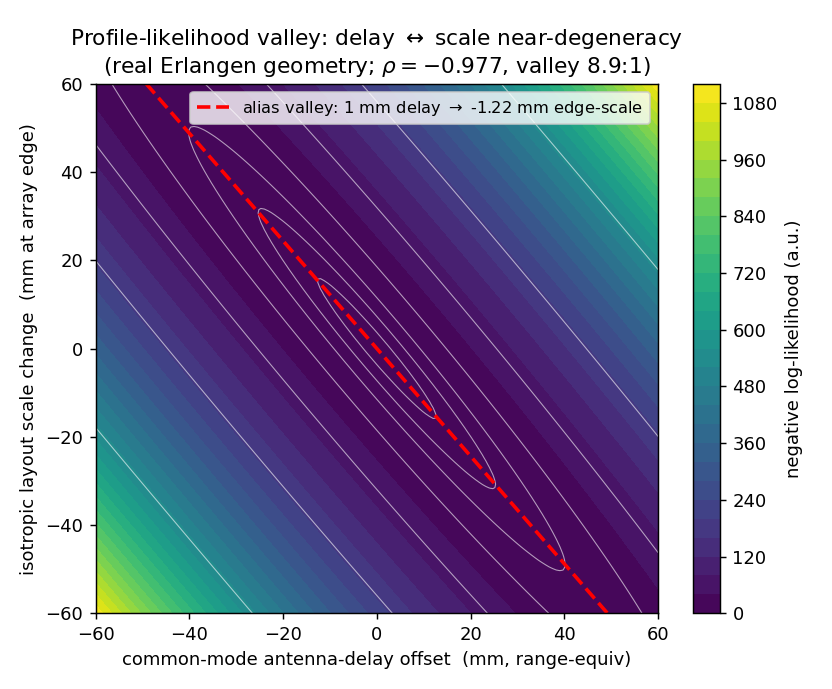
\includegraphics[width=0.62\textwidth]{literature_search/delay_scale_valley.png}
\caption{Profile-likelihood valley of the joint anchor self-calibration on the real
Erlangen geometry, projected onto the (common-mode antenna-delay, isotropic layout-scale)
plane (both axes in mm at the array edge). The long diagonal trough is the delay--scale
near-degeneracy: a common-mode delay is absorbed almost entirely as a layout-scale change
($\rho=-0.977$, variance inflation $22\times$, alias slope $1$~mm delay $\to -1.22$~mm
edge-scale). This is the anchor-side mechanism behind the wrong-geometry-wins paradox.}
\label{fig:valley}
\end{figure}

We separately examined whether the \emph{vertical}
component of the static error is an observability deficit or a delay effect; this
is a tag-side question, distinct from the anchor-side delay--scale direction
discussed above. The eight-anchor two-layer array already has well-conditioned
vertical geometry, so no observability deficit is expected; the self-calibration
vertical-CRLB analysis (derived in the companion system paper: singular for a single
coplanar layer, $\partial r/\partial y = 0$, falling to about $63$~mm for the balanced
four-plus-four array, essentially the production vertical error) confirms the vertical
geometry is at its observability floor, so the residual is not a geometry deficit. Instead, because every
tag observes the anchors with limited elevation diversity, a common-mode tag range
bias aliases predominantly into the vertical coordinate: a geometric
dilution-of-precision analysis of the deployment gives a vertical-to-horizontal
alias ratio of about seven and $\mathrm{VDOP}/\mathrm{HDOP}\approx1.6$, the UWB
analogue of the GPS receiver-clock/altitude coupling. As an independent empirical
check, an active vertical-information injection -- a tilted two-tag rotating arm
sweeping the rotation plane from horizontal to vertical during self-calibration --
did not reduce the recovered vertical error and showed no dose--response with
rotation tilt under either a free-point or a rigid-body arm model, confirming the
vertical error is dominated by this per-tag delay--altitude alias rather than by
anything additional vertical calibration data could supply (see the supplementary
experimental report).

This literature supports our Fisher/profile-likelihood language, but it does not remove the novelty. The Erlangen result is not just that a ranging network can be weakly identifiable. It is that a concrete range-only UWB self-calibration has a delay--layout direction whose in-environment winner changes when the tag-anchor positive range tail is reduced.

\subsection{Evaluation Methodology}

Several prior systems use ground truth, motion capture, or external trajectory sources for evaluation \citep{lutz_2019_visual_inertial_slam_uwb_error_model,ledergerber_2018_calibrating_away_inaccuracies_uwb,queralta_2020_uwb_based_system_for_uav}. What is less common is an explicit separation between anchor-side metric correctness and tag-side same-environment positioning accuracy. The Erlangen analysis uses Sim(3) scale, transfer matrices, winner's-curse correction, nested spatial validation, phase-center sensitivity, and raw-frame ranking reversal as separate checks. This is a measurement-validity protocol rather than a new real-time localization algorithm. All figures here derive from fixes (and an inter-anchor self-calibration) in which \textbf{all eight anchors of the 4+4 array participate}; the result is a property of that full-array participation, not of the ranging protocol---for a static fix the eight ranges are equivalent whether gathered sequentially or by broadcast. A reproduction that admits fixes from fewer anchors (e.g.\ a four-anchor subset) faces a much larger vertical CRLB or, for coplanar subsets, the singular regime, and is not expected to reproduce these numbers.

\subsection{Independent Observation of the Wrong-Calibration-Wins Paradox}

The delay--layout coupling documented in our Erlangen campaign is not unique to our
setup. Luder et al.\ recently reported that self-localized UWB anchor positions
produced better tag accuracy than laser-measured ground truth positions (13.96~cm
versus 16.57~cm average 2D error) in an outdoor 600~m$^2$ deployment using DWM3000
hardware \citep{luder_2025_anitrack}. The authors described the self-localized result as ``more accurate'' but did not
investigate the underlying cause. Their observation is \emph{consistent with} our
delay--layout interpretation, but we do not present it as confirmation: the reported
13.96 versus 16.57~cm difference is within one standard deviation over only seven tag
positions, and could equally arise from laser-survey error, 2D projection,
anchor-height handling, or environment-specific NLOS. We therefore cite AniTrack as an
independent external observation that motivates the question, not as a replication of
the mechanism, and not as evidence that the coupling is a general property.

\subsection{Generalization Beyond UWB}

We note, as a discussion-level conjecture rather than a contribution, that the
delay--layout coupling in this campaign resembles a broader identifiability pitfall in
ranging-based self-calibration: where a per-device nuisance parameter (device delay,
clock offset, sound speed) and a geometric parameter (layout scale) share a weakly
observable direction, structured bias can make the metric-incorrect (scale-biased) solution appear
empirically better. The analogy is imperfect and we flag its limit explicitly: antenna
delay enters the range model \emph{additively} (a constant offset) while layout scale
is \emph{multiplicative}, so the cancellation is only approximate over the deployment's
working-distance range and would mis-track if distances changed substantially. We
therefore treat GNSS clock--geometry and acoustic sound-speed--geometry as motivating
cross-domain analogies, not as evidence of generality, and we make no cross-domain
empirical claim.

\subsection{Cross-Domain Prior Art on Scale--Propagation-Parameter Coupling}

The scale--delay coupling identified in our campaign is not conceptually unique
to UWB. In acoustic microphone array self-calibration, Burgess, Kuang, and
\AA{}str\"om \citep{burgess_2015_toa_self_calibration} characterize the scale and
offset ambiguities in TOA/TDOA self-calibration as affine-subspace rank
deficiencies; Thrun \citep{thrun_2005_affine_structure_from_sound} recovers acoustic
geometry only up to an affine (scale-bearing) transform; Kuang and \AA{}str\"om
\citep{kuang_2013_stratified_tdoa_self_calibration} solve transmitter/receiver
geometry up to an unknown affine map before a metric upgrade; and Crocco et al.\
\citep{crocco_2012_bilinear_self_calibration} jointly self-calibrate sensor positions
and timing offsets. Critically for our framing, these works treat delay/offset as a
\emph{first-class jointly-solved unknown with formally characterized degeneracies},
not as a nuisance correction---so our claim is not that delay-as-unknown is new, but
that the UWB additive-delay \emph{in-environment cancellation} (where the absorbed
error helps positioning in the deployment environment) differs from their
affine/dimensional degeneracies. Within UWB, Batstone et al.\
\citep{batstone_2017_realtime_toa_uwb_self_calibration} already perform range-only TOA
anchor self-calibration, and recent UWB-inertial work that augments per-anchor
multiplicative scale and additive bias states jointly (e.g.\ MR-ULINS,
arXiv:2408.05719) is the closest parameterization to ours---though it does not
characterize the scale--delay pair as a weakly observable direction.
In cooperative wireless network localization, Shen, Wymeersch, and Win
\citep{shen_2010_fundamental_limits_cooperative} show that without sufficient
anchors the Fisher information matrix is rank-deficient due to geometric and
clock-related ambiguities. In GNSS, Pan et al.\
\citep{pan_2015_realtime_ppp_clock_orbit} demonstrate that satellite-clock
estimation can absorb part of the orbit error, and this error absorption
\emph{improves} positioning accuracy by 38.8\% and 36.1\% in their rover tests,
making it the closest cross-domain analog to ``error absorption helps
positioning.''

These works, together with the textbook bias--variance / shrinkage principle that a
deliberately biased model can lower prediction error
\citep{hastie_2009_elements_statistical_learning}, establish that the \emph{existence}
of a scale--propagation-parameter coupling and of useful-bias effects is prior art.
Our contribution is not the bare existence of the coupling, but its specific
manifestation in UWB anchor self-calibration: (i)~the weakly observable direction
between per-device antenna delay and global metric scale, indicated by common-mode
scale recovery and a cost-clamp test, now quantified by a gauge-free Fisher/profile-likelihood analysis ($\rho=-0.977$, $22\times$ variance inflation);
(ii)~the result that this coupling makes the scale-biased layout
\emph{outperform} the metric-correct one on same-environment positioning when the tag
delay is uncorrected---a UWB manifestation we did not find explicitly reported, while
acknowledging GNSS clock--orbit absorption \citep{pan_2015_realtime_ppp_clock_orbit}
and acoustic scale ambiguity \citep{burgess_2015_toa_self_calibration} as closely
related cross-domain precedents; and (iii)~the use of structured-range-bias reduction
as a diagnostic intervention to reveal the true calibration quality.

\section{Why the Coupling Has Not Been Identified Before}

The UWB positioning literature divides into two groups that rarely separate metric
correctness from in-environment accuracy, which is why delay--layout coupling is easy
to miss. We do not claim it \emph{cannot} be observed---only that the standard
evaluations do not surface it.

\textbf{Group 1: Anchor positions assumed known.} The majority of UWB positioning
papers treat anchor coordinates as pre-surveyed infrastructure
\citep{prorok_2013_models_algorithms_uwb_localization_thesis,wymeersch_2012_a_machine_learning_approach,kong_2023_nlos_identification_for_uwb,sung_2023_accurate_indoor_positioning_for}.
In this paradigm, geometry is fixed and delay is calibrated independently against
known distances. The two parameter spaces never interact in the same estimation
problem. Any delay--geometry coupling is invisible because there is no geometry to
couple with: the anchor positions are inputs, not outputs.

\textbf{Group 2: Anchor positions estimated.} A smaller body of work estimates
anchor positions from inter-anchor ranges, robot trajectories, or auxiliary sensing
\citep{hamer_2018_self_calibrating_ultra_wideband_network,ridolfi_2021_self_calibration_and_collaborati,herbruggen_2023_multihop_self_calibration_algori,piavanini_2022_a_calibration_method_for}.
These papers jointly estimate positions and sometimes delays, so the coupling can
in principle arise. However, they evaluate success by \emph{tag positioning accuracy},
not by \emph{metric correctness of the anchor geometry}. If the coupling produces a
scale-biased layout that cancels NLOS bias and gives low tag error, it is reported as
a successful calibration. Corbalan et al.\
\citep{corbalan_2023_self_localization_uwb_anchors} are a partial exception---they do
compare self-localized geometry against ground truth and report that geometry error
propagates only weakly to tag error---but they do not construct a case where the
scale-biased layout \emph{wins}, nor isolate a bias-cancellation cause. The
AniTrack result \citep{luder_2025_anitrack} is a
concrete example: self-localized anchors outperformed ground truth anchors on tag
accuracy, and the authors reported this as a positive outcome without
investigating the geometry.

\textbf{What is needed to observe the coupling.} Three conditions must be met
simultaneously: (1)~range-only anchor self-calibration, so that delay and geometry
can interact in the solver; (2)~external ground truth for the anchor geometry, so
that metric correctness can be evaluated independently of tag accuracy; and
(3)~comparison of multiple solver parameterizations, so that the ranking paradox
becomes visible. The Erlangen campaign satisfies all three. Most prior work
satisfies at most one.

\section{Novelty Gap Table}

\begin{table}[H]
\centering
\caption{Novelty gaps after full-text checking.}
\small
\begin{tabular}{@{}p{36mm}p{49mm}p{49mm}@{}}
\toprule
Topic & Prior art covers & Remaining gap addressed here \\
\midrule
UWB anchor self-calibration & Automatic anchor localization, robot-aided calibration, multihop calibration. & Same-environment accuracy can prefer a scale-biased layout. \\
Antenna delay calibration & Device delay, received-power bias, module-dependent range models. & Delay error is analyzed as coupled to layout scale, not only as a standalone nuisance. \\
NLOS mitigation & Classification, weighting, CIR/statistical features, learned corrections. & Range-bias reduction is used as an intervention that reverses the calibration ranking (reported separately). \\
Identifiability & Graph rigidity, observability, Fisher/CRB bounds. & The weak direction is interpreted physically as delay--layout coupling in a measured UWB campaign. \\
Evaluation & Ground truth and held-out experiments appear in individual systems. & Metric correctness, p50 accuracy, post-selection optimism, and dynamic transfer are separated explicitly. \\
Independent paradox observation & Self-localized anchors can sometimes outperform surveyed anchors in tag accuracy. & Why this happens, and whether it indicates a calibration quality problem rather than a calibration success. \\
Researcher-group split & UWB research divides into known-anchor positioning and self-calibration, evaluated by different criteria. & Neither group checks whether self-calibrated geometry is metrically correct and whether tag accuracy is a reliable proxy for calibration quality. \\
Cross-domain coupling & Scale--propagation-parameter coupling is known in acoustic and GNSS self-calibration, and GNSS error absorption can improve positioning. & The coupling interacts with structured range bias to make the scale-biased layout win in-environment, which has not been reported in prior ranging systems. \\
Generality & Other ranging systems know clock, bias, and geometry couplings. & The paper shows a concrete scale-bias cancellation failure mode (a scale-biased layout winning in-environment under an uncorrected tag delay) with Vicon-grounded evidence. \\
\bottomrule
\end{tabular}
\end{table}

\section{Our Contribution}

This paper makes two contributions that together form its headline: a Vicon-grounded
\emph{quantitative characterization} of the delay--layout coupling (we do not claim first
discovery of the qualitative effect), and a methodological \emph{falsification protocol} built on
it. We foreground the two jointly rather than ranking one above the other.

The first contribution is empirical. The qualitative observation that a common
delay offset trades off with geometric scale in ranging self-calibration has been
noted in acoustic/TOA array self-calibration \citep{burgess_2015_toa_self_calibration}; in UWB, the
closely related self-calibration of \citet{hamer_2018_self_calibrating_ultra_wideband_network} jointly
handles clock synchronization and anchor-position estimation. We provide
an explicit, Vicon-validated \emph{quantitative characterization} of this coupling in
UWB anchor self-calibration (we do not claim to be first to observe it, given the
cross-domain and AniTrack precedents above). A four-way ablation that crosses two layout sources (self-calibrated
\texttt{v4-io} coordinates, Vicon-measured coordinates) with residual-correction
treatments shows the fitted corrections are frame-conditioned: Vicon-measured anchor
coordinates give 311~mm RMSE with no correction and 252~mm with transplanted corrections,
but 78~mm once the corrections are re-estimated in the Vicon frame. A common-mode delay
re-parameterization ($d_i = c + e_i$, $c = 112$~mm) recovers metric scale from
inter-anchor ranges alone, moving the AutoPos-to-Vicon Sim(3) scale from 0.958 to 1.010
and the rigid anchor RMSE from 105.4 to 63.0~mm; clamping the common mode to zero raises
the solver cost by about 70\% and five perturbed initializations converge to the same
scale, indicating a weakly observable---not strictly degenerate---delay--scale
direction (now confirmed by the gauge-free Fisher analysis above: common-mode delay
correlates with isotropic layout scale at $\rho=-0.977$, a $22\times$ variance inflation).
We then show that the metric-correct common-mode layout is the worse same-environment
positioner (109.5~mm median) than the scale-biased \texttt{v4-io} layout (72.7~mm)
\emph{only when the tag delay is left uncorrected}: the scale-biased layout's scale error
compensates an uncorrected positive tag-device delay. The fair-comparison control points the same way: the physically honest correction is a \emph{single global}
tag-delay constant, because the deployed custom SS-TWR firmware applies one generic
antenna-delay default (the vendor example value, 16436 device units) identically to every
node---all eight anchors and the tag---with no per-device calibration, so the residual
per-device delays are exactly what the self-calibration absorbs into geometry. With a
leave-one-out, no-peek constant ($\approx 50$~mm, the median ranging residual on held-out
positions) the metric-correct layout becomes the better positioner: 68.5~mm held-out
median (P95 156~mm) versus 72.7~mm. The effect is carried by the paired comparison and the tail,
not by the marginal-median gap --- the $\sim$4~mm median difference has a paired bootstrap confidence
interval spanning zero, but across the 24 static positions the metric-correct layout is better at 17
(paired signed-rank $p\approx0.02$) and sharply reduces the error tail (RMSE 109.8 to 82.8~mm; P95
171.5 to 156~mm), whereas per-frame joint estimation only ties the median (72.9~mm) by overfitting and
blows the tail to P95 317.5~mm. This closes the causal chain: the scale-biased layout's apparent advantage
was an uncorrected constant the wrong geometry happened to absorb, not a genuine
superiority.

\textbf{The deeper reading: self-consistent is not metric.} Same-environment
accuracy cannot certify a calibration because the self-calibrated layout is internally
\emph{self-consistent} but not \emph{metric}. The common-mode delay and the isotropic
layout scale span a near-degenerate direction ($\rho=-0.977$), so a whole family of
(scale,~delay) solutions reproduces the inter-anchor ranges equally well; the range data
alone cannot select the metrically true member, and \texttt{v4-io} is simply the member
the solver happened to pick, its $4.4\%$ scale bias silently encoding the uncorrected
common-mode tag delay. It positions well only \emph{inside its own delay convention}:
correcting the geometry without also correcting the delay steps off the self-consistent
manifold, and the apparent advantage disappears. Selecting the metric member therefore
requires information outside the ranges---one known baseline, the factory common-mode
delay, or an external metric reference such as Vicon---to pin the degenerate scale
direction. This is also why the transfer claim must be earned rather than assumed:
sweeping the layout across rooms is precisely the lever that exercises the degenerate
direction and forces the true scale to reveal itself.

\textbf{Factory OTP does not supply the per-device delays.} A natural objection is that the
DWM1001C stores a factory antenna-delay calibration in DW1000 OTP, so applying it should remove the
per-device delay the coupling exploits. We read the OTP of all nine modules (eight anchors and the
static tag, one manufacturing lot) and verified the lone outlier with five repeated power-cycle reads.
The stored antenna delay is \emph{near-uniform} --- eight modules read 16472 device units and one
anchor (confirmed stable) reads 16451 --- and it does \emph{not} track the per-device delay the solver
must recover: the seven modules sharing the identical OTP value have fitted delay terms spanning
roughly $49$--$148$~mm, and the single genuine outlier's fitted term matches that of a same-OTP module
rather than reflecting its $21$-unit ($\approx 98$~mm) OTP offset. The per-device
antenna-calibration-temperature field is unprogrammed on every unit, indicating no per-device
antenna-delay calibration was performed --- although the same memory does carry per-device crystal-trim
and temperature-sensor references that vary unit to unit. Applying the OTP value is therefore a
near-uniform common-mode shift that only rescales the layout and cannot supply the per-device delay
differences that drive the coupling. The per-device delays are thus not recoverable from factory data --- only from
per-unit bench calibration (not done in deployment) or self-calibration, which
entangles them with geometry --- the effect studied here. The coupling is intrinsic to these commodity single-antenna modules (DWM1001C/DW1000), not an
artifact of a skipped calibration step.

The evidence chain is falsification-aware. The common-mode parameterization
absorbs bulk anchor delay and fixes scale, and the per-anchor range-bias decomposition
closes the error budget: eight positive per-device terms with mean 94.6~mm (anchor~A
largest at 148.2~mm) reproduce the measured pairwise excess to within 0.11~mm.
Phase-center sensitivity shows that the \texttt{v4-io}-over-common-mode static ranking
is robust to marker-offset perturbations beyond 10~mm, while the Vicon-oracle rank is
fragile near 2~mm and is therefore not used as the sole proof. The raw-frame
intervention that reduces the positive tag-anchor tail reverses the in-environment
ranking in favour of the metric-correct layout, providing the causal evidence that the
scale-biased layout's advantage came from cancellation rather than from a generally better
physical calibration.

The second contribution is methodological. We provide a Vicon-grounded
error-analysis protocol that separates metric correctness, same-environment
positioning accuracy, post-selection optimism, and dynamic transfer. The protocol
includes Sim(3) scale validation against Vicon, a transfer matrix over layout and
delay choices, winner's-curse correction, nested spatial cross-validation,
phase-center sensitivity analysis, NLOS leakage auditing, and ROTO gap
decomposition. This matters because a single-number accuracy report would have
called the \texttt{v4-io} layout the winner and hidden the physical reason---and indeed, the AniTrack
result \citep{luder_2025_anitrack} shows exactly this: without the falsification
protocol, the scale-bias cancellation phenomenon (a scale-biased layout winning in-environment) is reported as a success rather than
diagnosed as a coupling artifact.

\textbf{Priority, disclosure, and reproducibility.} We stake the flag not on the \emph{existence} of
the delay--layout coupling --- the acoustic, GNSS, and AniTrack precedents above forbid that claim ---
but on three things later UWB self-calibration work cannot route around. (i)~The first gauge-free
Fisher/profile-likelihood \emph{quantification} of the delay$\leftrightarrow$layout-scale
near-degeneracy on real UWB hardware: common-mode delay correlated with isotropic layout scale at
$\rho=-0.977$, a $22\times$ variance inflation, an alias of $1$~mm delay $\leftrightarrow -1.22$~mm
edge-scale ($-645$~ppm), with profile-likelihood valley elongation $8.9{:}1$. (ii)~The conditional
wrong-geometry-wins regime \emph{and} the control that closes it: a single global tag-delay constant
flips the in-environment ranking so the metric-correct layout becomes the better positioner at most
static positions ($68.5$ vs $72.7$~mm median; better at 17 of 24, paired $p\approx0.02$, with the error
tail cut from $171.5$ to $156$~mm P95), establishing
that the scale-biased layout's advantage was an uncorrected constant, not a better calibration.
(iii)~The Vicon-grounded falsification protocol that separates metric correctness from same-environment
accuracy. The enabling combination is stated once ---
range-only UWB anchor self-calibration $+$ independent metric (Vicon) ground truth for the
\emph{geometry} $+$ multiple solver parameterizations compared on that ground truth --- the exact
three-condition conjunction that prior work satisfies at most one of (\S\,``What is needed to observe
the coupling''). The Fisher derivation and figure ship as a runnable artifact, making the $\rho=-0.977$ / $22\times$ numbers
and the $0.958\!\to\!1.010$ scale recovery independently reproducible: a reusable artifact later UWB
self-calibration evaluations must cite to claim a self-calibrated layout is metrically correct, not
merely a good in-environment positioner. \emph{Citable priority sentence:}
\emph{``In range-only UWB anchor self-calibration the common-mode antenna-delay parameter is weakly
observable against isotropic layout scale --- measured at $\rho=-0.977$ ($22\times$ variance
inflation) on the deployed eight-anchor array --- so
same-environment tag accuracy can rank a scale-biased layout above a metric-correct one until a single
global delay constant is applied --- after which the metric-correct layout becomes the better positioner.''}

\section{Nearest Prior Art}

\begin{center}
\small
\begin{longtable}{@{}p{30mm}p{37mm}p{39mm}p{37mm}@{}}
\caption{Closest papers and specific differences.}\\
\toprule
Paper & What they specifically did & How our work differs & Why the difference matters \\
\midrule
\endfirsthead
\toprule
Paper & What they specifically did & How our work differs & Why the difference matters \\
\midrule
\endhead
\citet{lutz_2019_visual_inertial_slam_uwb_error_model} & Used visual-inertial SLAM and fiducial markers to estimate UWB anchor poses and sensor error-model parameters. & We analyze range-only self-calibration where delay and layout scale are weakly coupled, without using VINS as the calibration truth source. & Their method improves calibration with external visual structure; ours explains why a radio-only calibration can look better while being metric-incorrect (scale-biased). \\
\citet{hamer_2018_self_calibrating_ultra_wideband_network} & Built a self-calibrating one-way UWB network with clock synchronization and anchor position computation for multi-robot localization. & We focus on validation against Vicon and on the layout/delay/range-bias cancellation that lets a scale-biased self-calibrated layout outperform the metric-correct one in-environment. & A working self-calibrating network does not by itself tell whether the empirically best layout is physically correct. \\
\citet{luder_2025_anitrack} (AniTrack) & Deployed a self-localizing UWB system for animal tracking and found self-localized anchors outperformed laser-surveyed anchors in tag accuracy (13.96 vs 16.57 cm average error). & We explain why this can happen: delay--layout coupling lets a scale-biased self-calibrated layout cancel structured range bias. We validate with Sim(3) scale, a four-way layout/delay ablation, and common-mode scale recovery. & Their unexplained observation is consistent with our interpretation but is not a replication: the 13.96 vs 16.57~cm gap is within one standard deviation over seven positions and has competing explanations (survey error, 2D projection). We propose and Vicon-test a candidate mechanism. \\
\citet{pan_2015_realtime_ppp_clock_orbit} (GNSS) & Showed satellite-clock estimation absorbs orbit error, improving PPP positioning accuracy and convergence. & Their error absorption is clock-absorbs-orbit in GNSS, where satellite infrastructure is not self-calibrated by the rover. Our coupling is between self-calibrated anchor geometry and per-device delay, where a scale-biased layout cancels structured positive range bias. & They demonstrate that coupled-error absorption can help positioning. We show that it can make a metric-incorrect calibration win over the correct one when the tag bias is uncorrected. \\
\citet{ledergerber_2018_calibrating_away_inaccuracies_uwb} & Calibrated module-dependent delays and range inaccuracies by maximum likelihood, without external ground truth. & We show that improving a delay/range model is not the same as resolving scale coupling in anchor self-calibration. & Their result motivates range calibration; our result warns that calibration criteria can reward the wrong geometric solution. \\
\citet{shalaby_2023_calibration_and_uncertainty_char} & Proposed scalable antenna-delay calibration and received-power-dependent bias/uncertainty models. & We do not propose another delay estimator; we show delay estimates can interact with layout scale and structured NLOS. & It reframes delay from a standalone correction into a parameter that can hide a geometric error. \\
\citet{de_preter_2019_range_bias_modeling_autocalibration} & Modeled range bias and autocalibration in a UWB positioning system. & We test whether reducing structured range bias changes the calibration ranking, rather than only improving a biased range model. & This turns range-bias reduction into evidence about calibration validity. \\
\citet{difranco_2017_calibration_free_network_localization_nlos_uwb} & Localized a network from biased, multimodal NLOS UWB measurements without prior calibration. & We calibrate and compare physical layouts, including a metric-correct common-mode layout and a scale-biased \texttt{v4-io} layout. & Their NLOS robustness is not a test of whether a scale-biased layout can win under biased tag ranges. \\
\bottomrule
\end{longtable}
\end{center}

\section{Scope and Limitations}

\begin{table}[h]
\centering
\caption{Claims we do not make.}
\small
\begin{tabular}{@{}p{49mm}p{88mm}@{}}
\toprule
Not claimed & Reason \\
\midrule
CIR-free deployable NLOS classifier & The raw-frame lower-tail statistic is a separately reported static batch intervention, not a real-time classifier. \\
Real-time dynamic improvement & ROTO has one-frame ranges and remains around 101.5 mm under the conservative alignment. \\
Common-mode layout transfers better to new rooms & The scale argument suggests transfer, but an independent room is still needed. \\
Mixture-model superiority & The simple lower-tail statistic beat the tested mixtures in this dataset (reported separately). \\
20--30 mm UWB accuracy & The static median floor remains tens of millimetres and the P95 tail remains high. \\
Vicon oracle proves cancellation alone & Phase-center sensitivity makes that single argument fragile. \\
Rigid-body ROTO improvement & The tested two-tag rigid solvers worsened the dynamic result. \\
\bottomrule
\end{tabular}
\end{table}

\begin{thebibliography}{99}
\bibitem[Almansa et~al.(2020)]{almansa_2020_autocalibration_mobile_uwb_localization} Almansa, C.M., Shule, W., Queralta, J.P. and Westerlund, T., 2020. Autocalibration of a mobile UWB localization system for ad-hoc multi-robot deployments in GNSS-denied environments. \emph{arXiv preprint arXiv:2004.06762}.
\bibitem[Aspnes et~al.(2006)]{aspnes_2006_theory_network_localization} Aspnes, J., Eren, T., Goldenberg, D.K., Morse, A.S., Whiteley, W., Yang, Y.R., Anderson, B.D.O. and Belhumeur, P.N., 2006. A theory of network localization. \emph{IEEE Transactions on Mobile Computing}, 5(12), pp.1663--1678.
\bibitem[Batstone et~al.(2017)]{batstone_2017_realtime_toa_uwb_self_calibration} Batstone, K., Oskarsson, M. and \AA{}str\"om, K., 2017. Towards real-time time-of-arrival self-calibration using ultra-wideband anchors. In: \emph{2017 International Conference on Indoor Positioning and Indoor Navigation (IPIN)}. IEEE, pp.1--8. DOI: 10.1109/IPIN.2017.8115885.
\bibitem[Burgess et~al.(2015)]{burgess_2015_toa_self_calibration} Burgess, S., Kuang, Y. and \AA{}str\"om, K., 2015. TOA sensor network self-calibration for receiver and transmitter spaces with difference in dimension. \emph{Signal Processing}, 107, pp.33--42.
\bibitem[Corbalan et~al.(2023)]{corbalan_2023_self_localization_uwb_anchors} Corbalan, P., Picco, G.P., Coors, M. and Jain, V., 2023. Self-localization of ultra-wideband anchors: From theory to practice. \emph{IEEE Access}, 11, pp.29711--29725.
\bibitem[Crocco et~al.(2012)]{crocco_2012_bilinear_self_calibration} Crocco, M., Del Bue, A. and Murino, V., 2012. A bilinear approach to the position self-calibration of multiple sensors. \emph{IEEE Transactions on Signal Processing}, 60(2), pp.660--673.
\bibitem[De Preter et~al.(2019)]{de_preter_2019_range_bias_modeling_autocalibration} De Preter, A., Goysens, G., Anthonis, J., Swevers, J. and Pipeleers, G., 2019. Range bias modeling and autocalibration of a UWB positioning system. In: \emph{International Conference on Indoor Positioning and Indoor Navigation (IPIN)}, pp.1--8.
\bibitem[Di Franco et~al.(2017)]{difranco_2017_calibration_free_network_localization_nlos_uwb} Di Franco, C., Prorok, A., Atanasov, N., Kempke, B., Dutta, P., Kumar, V. and Pappas, G.J., 2017. Calibration-free network localization using non-line-of-sight UWB measurements. In: \emph{ACM/IEEE International Conference on Information Processing in Sensor Networks (IPSN)}.
\bibitem[Goudar et~al.(2021)]{goudar_2021_online_spatiotemporal_calibration_uwb_imu} Goudar, A., Zhao, W. and Schoellig, A.P., 2021. Online spatio-temporal calibration of tightly-coupled ultrawideband-aided inertial localization. In: \emph{IEEE/RSJ International Conference on Intelligent Robots and Systems (IROS)}.
\bibitem[Guvenc et~al.(2007)]{guven_2007_nlos_identification_and_weight} Guvenc, I., Chong, C.-C., Watanabe, F. and Inamura, H., 2007. NLOS identification and weighted least-squares localization for UWB systems using multipath channel statistics. \emph{EURASIP Journal on Advances in Signal Processing}, 2007.
\bibitem[Hastie et~al.(2009)]{hastie_2009_elements_statistical_learning} Hastie, T., Tibshirani, R. and Friedman, J., 2009. \emph{The Elements of Statistical Learning: Data Mining, Inference, and Prediction}. 2nd ed. Springer.
\bibitem[Hamer \& D'Andrea(2018)]{hamer_2018_self_calibrating_ultra_wideband_network} Hamer, M. and D'Andrea, R., 2018. Self-calibrating ultra-wideband network supporting multi-robot localization. \emph{IEEE Access}, 6, pp.22292--22304.
\bibitem[Van Herbruggen et~al.(2023)]{herbruggen_2023_multihop_self_calibration_algori} Van Herbruggen, B., Luchie, S., Fontaine, J. and De Poorter, E., 2023. Multihop self-calibration algorithm for ultra-wideband anchor node positioning. \emph{IEEE Journal of Indoor and Seamless Positioning and Navigation}.
\bibitem[Hesch et~al.(2014)]{hesch_2014_camera_imu_observability} Hesch, J.A., Kottas, D.G., Bowman, S.L. and Roumeliotis, S.I., 2014. Camera-IMU-based localization: Observability analysis and consistency improvement. \emph{The International Journal of Robotics Research}, 33(1), pp.182--201.
\bibitem[Jeong et~al.(2023)]{jeong_2023_hybrid_quantum_convolutional_neu} Jeong, S.-G., Do, Q.-V., Hwang, H.-J., Hasegawa, M., Sekiya, H. and Hwang, W.-J., 2023. Hybrid quantum convolutional neural networks for UWB signal classification. \emph{IEEE Access}.
\bibitem[Jourdan et~al.(2008)]{joudarwin_2008_position_error_bound_uwb} Jourdan, D.B., Dardari, D. and Win, M.Z., 2008. Position error bound for UWB localization in dense cluttered environments. \emph{IEEE Transactions on Aerospace and Electronic Systems}, 44(2), pp.613--628.
\bibitem[Kong(2023)]{kong_2023_nlos_identification_for_uwb} Kong, Q., 2023. NLOS identification for UWB positioning based on IDBO and convolutional neural networks. \emph{IEEE Access}.
\bibitem[Kuang \& \AA{}str\"om(2013)]{kuang_2013_stratified_tdoa_self_calibration} Kuang, Y. and \AA{}str\"om, K., 2013. Stratified sensor network self-calibration from TDOA measurements. In: \emph{21st European Signal Processing Conference (EUSIPCO)}.
\bibitem[Ledergerber et~al.(2015)]{ledergerber_2015_robot_self_localization_one_way_uwb} Ledergerber, A., Hamer, M. and D'Andrea, R., 2015. A robot self-localization system using one-way ultra-wideband communication. In: \emph{IEEE/RSJ International Conference on Intelligent Robots and Systems (IROS)}, pp.3131--3137.
\bibitem[Ledergerber \& D'Andrea(2018)]{ledergerber_2018_calibrating_away_inaccuracies_uwb} Ledergerber, A. and D'Andrea, R., 2018. Calibrating away inaccuracies in ultra wideband range measurements: A maximum likelihood approach. \emph{IEEE Access}, 6, pp.78719--78730.
\bibitem[Liu et~al.(2024)]{liu_2024_data_driven_antenna_delay_calibr} Liu, Z., Hakala, T., Hyyppa, J., Kukko, A., Kaartinen, H. and Chen, R., 2024. Data-driven antenna delay calibration for UWB devices for network positioning. \emph{IEEE Transactions on Instrumentation and Measurement}.
\bibitem[Lutz et~al.(2019)]{lutz_2019_visual_inertial_slam_uwb_error_model} Lutz, P., Schuster, M.J. and Steidle, F., 2019. Visual-inertial SLAM aided estimation of anchor poses and sensor error model parameters of UWB radio modules. In: \emph{International Conference on Advanced Robotics (ICAR)}, pp.739--746.
\bibitem[Luder et~al.(2025)]{luder_2025_anitrack} Luder, V., Schulthess, L., Cortesi, S., Rivero Davis, L. and Magno, M., 2025. AniTrack: A power-efficient, time-slotted and robust UWB localization system for animal tracking in a controlled setting. \emph{arXiv preprint arXiv:2506.00216}.
\bibitem[Marano et~al.(2010)]{maran_2010_nlos_identification_and_mitigati} Marano, S., Gifford, W.M., Wymeersch, H. and Win, M.Z., 2010. NLOS identification and mitigation for localization based on UWB experimental data. \emph{IEEE Journal on Selected Areas in Communications}.
\bibitem[Meghani et~al.(2019)]{meghani_2019_empirical_based_ranging_error} Meghani, S.K., Asif, M., Awin, F. and Tepe, K., 2019. Empirical based ranging error mitigation in IR-UWB: A fuzzy approach. \emph{IEEE Access}.
\bibitem[Pan et~al.(2015)]{pan_2015_realtime_ppp_clock_orbit} Pan, S., Chen, W., Jin, X., Shi, X. and He, F., 2015. Real-time PPP based on the coupling estimation of clock bias and orbit error with broadcast ephemeris. \emph{Sensors}, 15(7), pp.17808--17826.
\bibitem[Patwari et~al.(2005)]{patwari_2005_locating_the_nodes} Patwari, N., Ash, J.N., Kyperountas, S., Hero, A.O., Moses, R.L. and Correal, N.S., 2005. Locating the nodes: Cooperative localization in wireless sensor networks. \emph{IEEE Signal Processing Magazine}, 22(4), pp.54--69.
\bibitem[Piavanini et~al.(2022)]{piavanini_2022_a_calibration_method_for} Piavanini, M., Barbieri, L., Brambilla, M., Cerutti, M., Ercoli, S., Agili, A. and Nicoli, M., 2022. A calibration method for antenna delay estimation and anchor self-localization in UWB systems. In: \emph{IEEE International Workshop on Metrology for Industry 4.0 \& IoT (MetroInd4.0\&IoT)}, pp.173--177.
\bibitem[Prorok(2013)]{prorok_2013_models_algorithms_uwb_localization_thesis} Prorok, A., 2013. \emph{Models and Algorithms for Ultra-Wideband Localization in Single- and Multi-Robot Systems}. PhD thesis. EPFL.
\bibitem[Queralta et~al.(2020)]{queralta_2020_uwb_based_system_for_uav} Queralta, J.P., Almansa, C.M., Schiano, F., Floreano, D. and Westerlund, T., 2020. UWB-based system for UAV localization in GNSS-denied environments. In: \emph{IEEE/RSJ International Conference on Intelligent Robots and Systems (IROS)}.
\bibitem[Ridolfi et~al.(2021)]{ridolfi_2021_self_calibration_and_collaborati} Ridolfi, M., Kaya, A., Berkvens, R., Weyn, M., Joseph, W. and De Poorter, E., 2021. Self-calibration and collaborative localization for UWB positioning systems. \emph{ACM Computing Surveys}.
\bibitem[Shah et~al.(2021)]{shah_2021_antenna_delay_calibration_of} Shah, S., Chaiwong, K., Kovavisaruch, L., Kaemarungsi, K. and Demeechai, T., 2021. Antenna delay calibration of UWB nodes. \emph{IEEE Access}, 9, pp.63294--63305.
\bibitem[Shah et~al.(2022)]{shah_2022_node_calibration_in_uwb_based} Shah, S., Kovavisaruch, L., Kaemarungsi, K. and Demeechai, T., 2022. Node calibration in UWB-based RTLSs using multiple simultaneous ranging. \emph{Sensors}, 22(3), 864.
\bibitem[Shalaby et~al.(2023)]{shalaby_2023_calibration_and_uncertainty_char} Shalaby, M., Cossette, C.C., Forbes, J.R. and Le Ny, J., 2023. Calibration and uncertainty characterization for ultra-wideband two-way-ranging measurements. In: \emph{IEEE International Conference on Robotics and Automation (ICRA)}.
\bibitem[Shen et~al.(2010)]{shen_2010_fundamental_limits_cooperative} Shen, Y., Wymeersch, H. and Win, M.Z., 2010. Fundamental limits of wideband localization---Part II: Cooperative networks. \emph{IEEE Transactions on Information Theory}, 56(10), pp.4981--5000.
\bibitem[Shi et~al.(2019)]{shi_2019_anchor_self_localization_algorit} Shi, Q., Zhao, S., Cui, X., Lu, M. and Jia, M., 2019. Anchor self-localization algorithm based on UWB ranging and inertial measurements. \emph{Tsinghua Science and Technology}.
\bibitem[Sung et~al.(2023)]{sung_2023_accurate_indoor_positioning_for} Sung, S., Kim, H. and Jung, J.-i., 2023. Accurate indoor positioning for UWB-based personal devices using deep learning. \emph{IEEE Access}.
\bibitem[Thrun(2005)]{thrun_2005_affine_structure_from_sound} Thrun, S., 2005. Affine structure from sound. In: \emph{Advances in Neural Information Processing Systems (NIPS)}, 18.
\bibitem[Venkatesh \& Buehrer(2007)]{venkatesh_2007_non_line_of_sight_identification} Venkatesh, S. and Buehrer, R.M., 2007. Non-line-of-sight identification in ultra-wideband systems based on received signal statistics. \emph{IET Microwaves, Antennas \& Propagation}.
\bibitem[Wymeersch et~al.(2009)]{wymeersch_2009_cooperative_localization_wireless_networks} Wymeersch, H., Lien, J. and Win, M.Z., 2009. Cooperative localization in wireless networks. \emph{Proceedings of the IEEE}.
\bibitem[Wymeersch et~al.(2012)]{wymeersch_2012_a_machine_learning_approach} Wymeersch, H., Marano, S., Gifford, W.M. and Win, M.Z., 2012. A machine learning approach to ranging error mitigation for UWB localization. \emph{IEEE Transactions on Communications}.
\bibitem[Yang et~al.(2024)]{yang_2024_uwb_nlos_identification_and} Yang, H., Wang, Y., Seow, C., Sun, M. and Plets, D., 2024. UWB NLOS identification and mitigation based on bidirectional encoder representations from transformer (BERT) deep learning. In: \emph{International Conference on Indoor Positioning and Indoor Navigation (IPIN)}.
\bibitem[Yogesh et~al.(2024)]{yogesh_2024_novel_calibration} Yogesh, V., Grevinga, L., Voort, C., Buurke, J.H., Veltink, P.H. and Baten, C.T.M., 2024. Novel calibration method for improved UWB sensor distance measurement in the context of application for 3D analysis of human movement. \emph{Engineering Science and Technology, an International Journal}, 58, 101844.
\end{thebibliography}

\end{document}
